\documentclass[../main.tex]{subfiles}

\begin{document}

\begin{figure}[H]
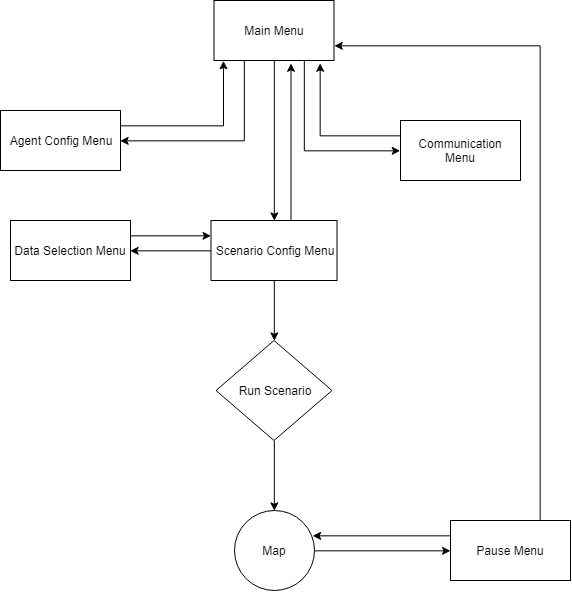
\includegraphics[width=\textwidth,height=\textheight,keepaspectratio]{MenuFlow.jpg}
\caption{Menu Flow}
\end{figure}

The menus system connects five setup menus and a pause menu allowing users to navigate between the entry point (the main menu) and the initiation/maintanance of a simulation. The flow of this menu structure can be seen in Menu Figure 1. with rectangles representing menus (widgets), diamonds representing actions and ovals representing maps.

\begin{figure}[H]
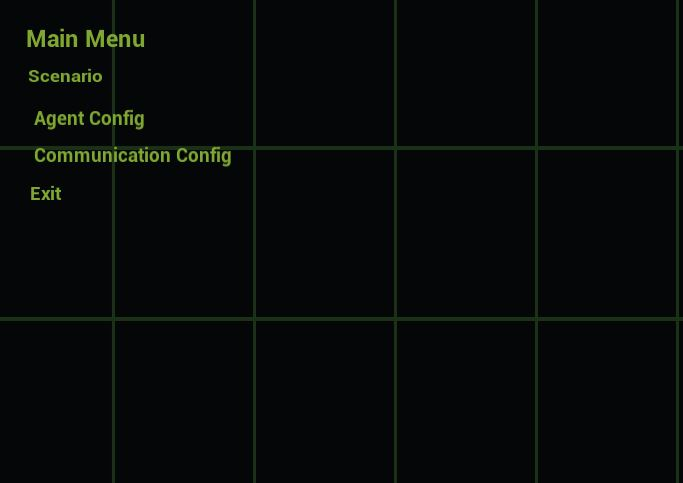
\includegraphics[width=\textwidth,height=\textheight,keepaspectratio]{MainMenu.jpg}
\caption{Main Menu}
\end{figure}

\break

\section{Main Menu}
The main menu is the entry point of the menu flow, it can be opened by playing any map using the MainMenuHUD. This is the default HUD for OpenerMap and so acts as an easy way to open up the menu flow for a user. The main menu has four options, Scenario, Agent Config, Communication Config and Exit.

The first three options will open up the corresponding menus and allowing the user to edit the scenario settings, specific agent configuration settings and communication settings respectively. The last option "Exit" will immediately terminate the program and acts as the exit point for the program.

\begin{figure}[H]
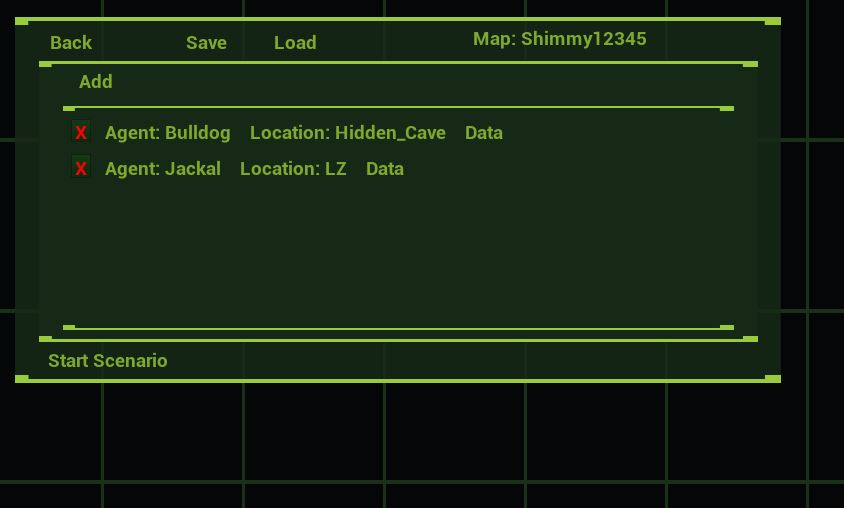
\includegraphics[width=\textwidth,height=\textheight,keepaspectratio]{ScenarioMenu.jpg}
\caption{Scenario Menu}
\end{figure}

\section{Scenario Config Menu}
The scenario config menu has five points of interest:

\begin{enumerate}
\item Back button, top left of screen. This button is used to return the the previous menu.
\item Map selection button, top right of screen. This button opens a drop down menu and allows users to select the map to be used in the scenario
\item Add button, below the Back button. This button adds a new blank spawn configuration.
\item Spawn configuration, below the Add button. These configurations allow the user to choose the agent to spawn and the location where the agent should be spawned. The included data button allows the user to open another menu and select what data to record from the agent once it's spawned.
\item Start button, bottom left of the screen. This button allows the user to run the scenario as configured.
\end{enumerate}

\begin{figure}[H]
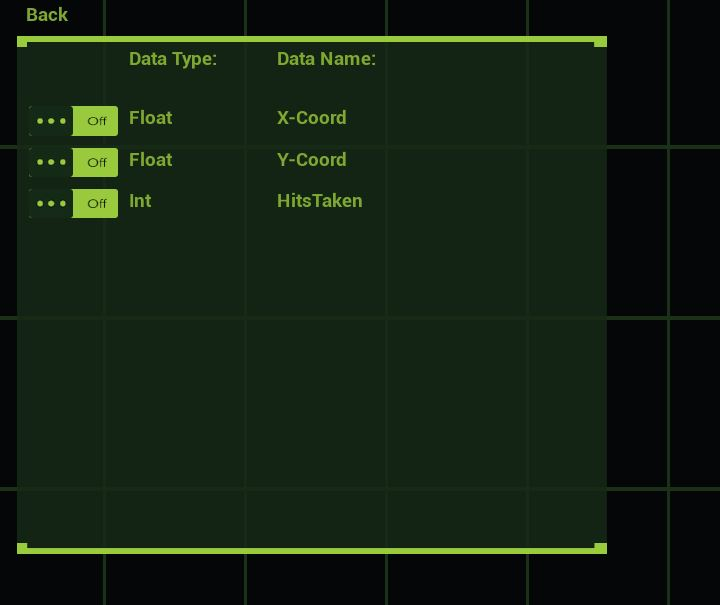
\includegraphics[width=\textwidth,height=\textheight,keepaspectratio]{DataMenu.jpg}
\caption{Data Menu}
\end{figure}

\section{Data Menu}
The data menu allows users to toggle on and off the data to be recorded for a given agent spawn. To toggle a data stream click the slider to the left of the streams data type.

\begin{figure}[H]
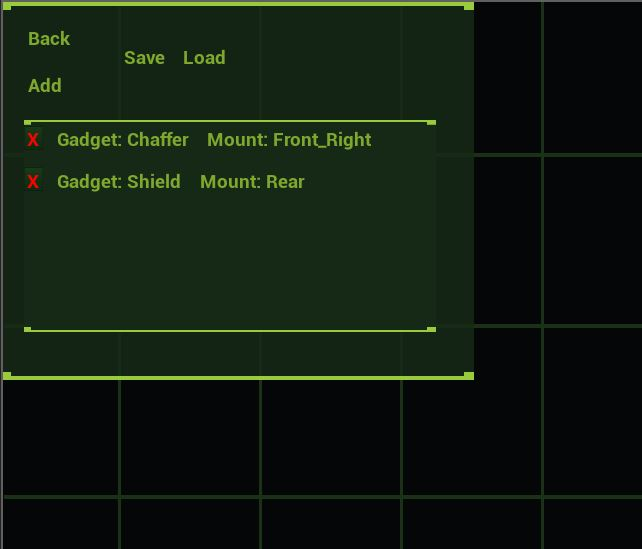
\includegraphics[width=\textwidth,height=\textheight,keepaspectratio]{AgentMenu.jpg}
\caption{Agent Menu}
\end{figure}

\section{Agent Menu}
The agent menu allows the user to configure an agent by adding and removing gadgets from mounting spots on existing agent blueprints. To add a gadget press the add button, select the gadget to mount and the mounting location.

\begin{figure}[H]
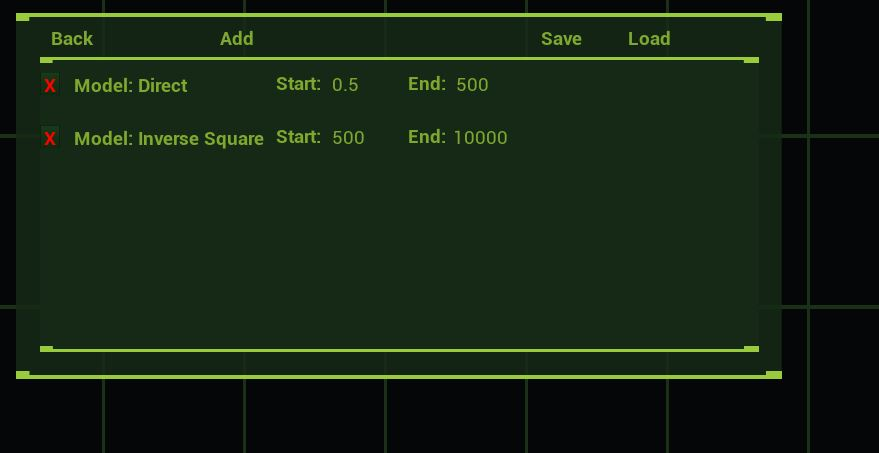
\includegraphics[width=\textwidth,height=\textheight,keepaspectratio]{ComMenu.jpg}
\caption{Communication Menu}
\end{figure}

\textbf{5. Communication Menu}
The communication menu allows users to add and remove frequency ranges and the models which should be used to propogate messages inside a scenario. Ranges can be added and removed using the coresponding buttons, the range values are in hertz.

\break

\begin{figure}[H]
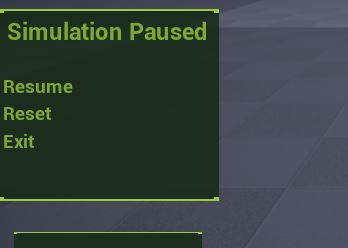
\includegraphics[width=\textwidth,height=\textheight,keepaspectratio]{PauseMenu.jpg}
\caption{Pause Menu.}
\end{figure}

\section{Pause Menu}
The pause menu is used to navigate in game functionality for the user, it can opened by pressing the pause key (default p) while using the TestbedPlayerController.


\end{document}
